\chapter{Implementation}

It would be very difficult to attempt to build a complete working system
during the course of the project, and that would be wholly out of scope. So
throughout this project, the idea has been to build prototypes that
demonstrate that a fully production-ready solution is viable.

\todo[inline]{Expand on this chapter intro}

\section{Developing the Base Station Code}
The main base station program is just a \acrshort{tcp} server that handles
commands coming in from the camera and motion sensors over the \gls{6lowpan}
connection. Since the Linux kernel can already handle the \gls{6lowpan}
connection, and no other hardware interfaces are required, there was a lot of
flexibility in the choice of language and framework used to build the server.
The Python language ended up being the choice of language, for its ease of
development and pseudocode-like syntax.

The core language library also includes the \texttt{socket} library, which
provides an easy to use, low-level interface for opening and accepting UDP
and \acrshort{tcp} connections. The server has a global dictionary that maps
the id numbers of sensor pairs to the id of a camera sensor and the id of a
motion sensor. This dictionary is populated from sensors which send an
identification (\texttt{id}) command, broadcasting their unique
\texttt{sensor\_id} and their \texttt{pair\_id}. This means that, when a
motion sensor sends a motion detection command to the server, the server can
look up the ID of the camera associated with the motion sensor and send it a
command to capture a photo.

The source code for the base station server is available in section
\ref{code:base-main} \textit{(page \pageref{code:base-main})}.

\section{Developing Remote Sensor Code}
The \gls{6lowpan} clicker that the motion and camera sensors use runs on a
\acrfull{rtos} called \textit{Contiki}~\cite{contiki}. The code that runs on
these devices has to be flashed to the onboard flash memory. Therefore,
Creator provide their own toolchain for compiling and flashing user code.
This, however, was extremely difficult to set up, and a lot of time was spent
obtaining the tooling, attempting to install the code, and being able to
access the clicker from my computers. A lot of documentation was missing or
not provided, which made independent investigations into the source code
necessary.

Another issue was with writing the sensor code itself. The only provided
documentation for Contiki is a handful of examples on its source code
repository, as well as a tutorial on the Creator
website~\cite{clickersetupguide}. To complicate matters further, the code
used to program the boards is a modified version of the C language, except
code runs in ``process threads''. However, after a lot of searching on the
web, the Contiki wiki was discovered~\cite{contiki-wiki}. Despite being
incredibly technical, there was helpful pieces of information available there
to help decipher the inner workings of the Contiki platform, notably how the
``protothreads'' work.

Debugging the code was a further complication when developing the sensor
code. The \gls{6lowpan} clicker only has a single MicroUSB port, which is
used for flashing code to the onboard memory, and does not have a USB port of
any kind to connect a serial terminal to. There is only two ways of debugging
the clicker\textemdash{}sending text over the \gls{6lowpan} connection, or
setting the two hardware LEDs on or off. A \acrshort{udp}-based debugging
server is available along with a \texttt{PRINTF} macro, however these did not
appear to work very well, if at all. It was also found that the debugging
server would not work if the device was making a separate connection to the
base station, such as when sending motion commands.

\subsection{6LoWPAN issues}
A reoccurring issue throughout the development of the remote sensors was the
reliability of the \gls{6lowpan} connection. It often took multiple minutes
or more for the remote sensors to connect to the base station, regardless of
whether it was a \acrshort{tcp} connection or a \acrshort{udp} connection.
Sometimes, the devices would not connect at all, and the debugging server
(when it worked) reported multiple dropped messages. Since the Ci40 uses the
2.4 \acrshort{ghz} frequency band, which is shared with many WiFi standards
as well as Bluetooth, there is a possibility that this might be caused by
interference between these devices, especially since all of the testing
environments available during this project were in close proximity to WiFi
links as well as Bluetooth devices, despite best efforts.

A manual published by \textit{NXP Semiconductors} highlights the issues that
can occur from the co-existence of these technologies on the same 2.4
\acrshort{ghz} frequency band~\cite{nxp2013ieee802154coexistence}. Notably,
on page 19, they recommend that ``to achieve satisfactory IEEE 802.15.4
[6LoWPAN] performance in the presence of WLAN interference, a channel
centre-frequency offset of 7 MHz is recommended'', and if \gls{6lowpan} is
running on the same channel as the WiFi link, ``a physical separation from
the WLAN \acrfull{ap} of 8 m is recommended''. Essentially, they recommend
either conducting radio operations away from WiFi \acrshort{ap}, or selecting
a different channel if possible. However, the WiFi \acrshort{ap}s in the
testing environment are managed by a third party, so it was not possible to
change their channels. Additionally, the documentation for the Ci40 base
station was not clear enough on whether it was possible to set the
\gls{6lowpan} wireless channel or not.

As a result of these \gls{6lowpan} issues, some modifications were made to
the project. The camera sensor would be prototyped by installing the camera
module \textit{directly} onto the Ci40 base station, to make development and
debugging easier. Since the Ci40 runs a full Linux operating system and full
WiFi stack, it is possible to connect to it using an \acrfull{ssh}
connection. In addition to this, code designed to run on the camera clicker
was not developed because it would be extremely similar to the motion sensor
code, albeit with the camera processing code instead of the motion sensor
event handling code.

\subsection{Working With The Camera Click Module}
One of the biggest obstacles during the project was working with the
\textit{MikroElektronika Camera Click} module~\cite{cameraclick}, to be used
as part of the prototype hardware for the remote camera sensor. The only
documentation provided for this sensor is available on their ``LibStock''
website~\cite{cameraclickexamples}, but the only documentation provided is a
board schematic and a code example, designed to be used with
\textit{MikroElektronika}'s own TFT display, with its own proprietary image
format.

However, the code example provided was enough to discover roughly how the
camera click board works and responds to input. It uses the \acrshort{spi}
interface to receive commands and send a new or buffered image back to the
parent device. The commands supported are, according to the code examples:

\begin{itemize}
  \item \texttt{\_\_CMD\_WRITE\_REG} (assumed) write to the registers on the
  camera \acrfull{mcu}, to set things like exposure and brightness settings.
  \item \texttt{\_\_CMD\_READ\_REG} (assumed) read from the registers on the
  camera \acrshort{mcu}.
  \item \texttt{\_\_CMD\_GET\_FRAME} capture a new photo and prepare to send
  it back through the \acrshort{spi} interface.
  \item \texttt{\_\_CMD\_GET\_FRAME\_BUFFERED} (assumed) get the currently
  buffered image from the camera, without capturing a new image.
  \item \texttt{\_\_CMD\_SET\_ROW\_NUM} unknown.
  \item \texttt{\_\_CMD\_SET\_ROW\_SIZE} unknown.
\end{itemize}

\subsubsection{The \acrshort{spi} Interface}
The \acrshort{spi} involves one ``primary'' device, which sends commands to
one or more ``secondary'' devices. There is four data lines involved:

\begin{itemize}
  \item CS\textemdash{}Chip Select. Selects the secondary device to use.
  \item MISO\textemdash{}Transmits data from the primary device to the
  secondary device.
  \item MOSI\textemdash{}Transmits data from the secondary device to the
  primary device.
  \item CLK\textemdash{}Timing signal.
\end{itemize}

The primary and secondary devices transmit data as if they were one
``rotary'' system. Each side has a buffer of a fixed size (in the case of the
camera module, 8 bits), and as the primary device pushes a bit to the
\acrshort{spi} interface, the secondary device sends a bit back. This
continues until the buffers are essentially swapped around.\todo{add SPI
diagram} One peculiarity in this implementation of \acrshort{spi} is that
the camera module use sa separate ``interrupt'' pin (provided by the
\gls{mikrobus} standard) to let the primary device know that it is ready for
commands.

\subsubsection{Getting Camera Output}
The code in Section~\ref{code:camera-base} shows the code used to attempt to
obtain output from the camera sensor, installed onto one of the Ci40's
\gls{mikrobus} ports. It works by initialising the \acrshort{spi} pins and
setting speed and other settings, before waiting for the camera to send a
``ready'' signal and then sending the \acrshort{spi} command to get an image
from the camera. It then reads the incoming data to a buffer, and saves that
buffer to a file. The data \textit{should}, in theory, be the image data from
the camera. This code should work since it roughly follows the steps used in
\textit{MikroElektronika}'s example code. However, the camera module
frequently returns a lot of blank data. Below is one example of data received
from the camera sensor after sending a \texttt{\_\_CMD\_GET\_FRAME} command:

\begin{verbatim}
  [mbell@chancery-lane ~]$ hexdump ~/out.bin
  0000000 ffff ffff ffff ffff ffff ffff ffff ffff
  *
  000c600 0000 0000 0000 0000 c611               
  000c60a
\end{verbatim}

\subsubsection{Interpreting Camera Output}
Sometimes the camera would send data that was not just a stream of \texttt{1}
bits, however it was not clear whether the returned data was nonsense, or if
the data was in some proprietary data format.

Figure~\ref{fig:yuvimage} shows the data previewed as a \textit{YUV} image.
This is an 8-bit pixel encoded image format that contains three values for
each colour\textemdash{}the brightness (also called luminance), and two
values defining the colour itself (the chroma)~\cite{softpixelyuv}. The data
was estimated to be using some kinda of YUV format, because of reoccurring
patterns in the data that suggested that pixel data was set as some 4-bit
value, then two 2-bit values.

The possibility of the data being stored as \acrfull{rgb} data was ruled out
when attempting to parse the raw image file as such. The results can be seen
in figure~\ref{fig:rgbimage}. It is clear that the data is not \acrshort{rgb}
since the rendering software runs out of bits roughly two-thirds of the way
through parsing the image. Since public access to the source code for the
camera module was prohibited by the manufacturer, it was impossible to tell
whether the image format chosen was incorrect, or if the camera module itself
was defective or damaged. Therefore, no image was ever able to be correctly
obtained from the camera module.

\begin{figure}
  \centering
  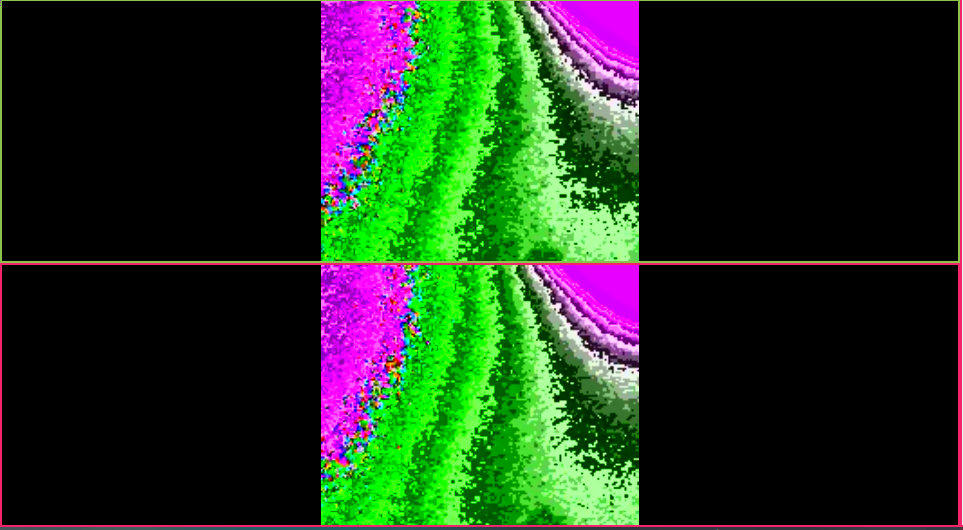
\includegraphics[width=0.8\textwidth]{cameraoutput1}
  \caption{The data received from the camera sensor, interpreted as a YUV-formatted image.}
  \label{fig:yuvimage}
\end{figure}

\begin{figure}
  \centering
  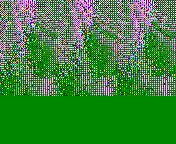
\includegraphics[width=0.8\textwidth]{cameraoutput2}
  \caption{The data received from the camera sensor, interpreted as a RGB-formatted raw image.}
  \label{fig:rgbimage}
\end{figure}

\subsubsection{Read-Only Register Random Number Generator}
The camera module used on the camera sensor is the OV7670-VL2A CMOS sensor,
and a datasheet is readily available online~\cite{omnivisiondatasheet}.